\definecolor{myyellow}{rgb}{1,0.96,0.49}
\chapter{Desarrollo}

\lstset{backgroundcolor=\color{myyellow}}
\lstinputlisting[language=Java,firstline = 1, lastline=51]{../src/CA.js}

\newpage

%\lstset{backgroundcolor=\color{myyellow}}

\lstset{inputencoding=utf8/latin1}
\lstinputlisting[language=Java,firstline = 1,lastline=51]{../mapExample/code.js}

\chapter{Resultados}

Por lo que una vez teniendo resultados esperados lo siguiente a realizar será extender el paradigma a otros modelos como SIRS, SEIR, etc.


%\section{}
% análisis
% Graficación
% Tabla rubrica

%
%\begin{figure}[h]
%	\centering
%	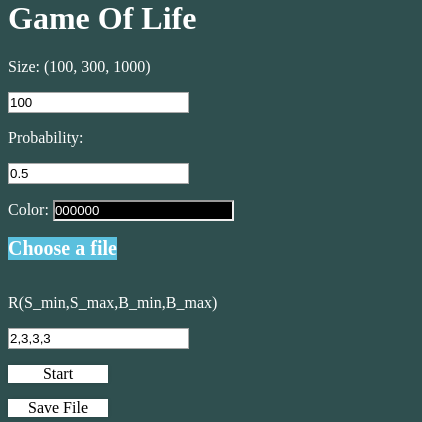
\includegraphics[width=0.7\textwidth]{capitulo2/images/menu.png}
%	\caption{Parámetros del programa}
%	\label{fig:menu}
%\end{figure}
%\newpage
